\documentclass[a4paper,12pt,twoside]{memoir}

% Castellano
\usepackage[spanish,es-tabla]{babel}
\selectlanguage{spanish}
\usepackage[utf8]{inputenc}
\usepackage[T1]{fontenc}
\usepackage{lmodern} % scalable font
\usepackage{microtype}
\usepackage{placeins}

\RequirePackage{booktabs}
\RequirePackage[table]{xcolor}
\RequirePackage{xtab}
\RequirePackage{multirow}

% Links
\PassOptionsToPackage{hyphens}{url}\usepackage[colorlinks]{hyperref}
\hypersetup{
	allcolors = {red}
}

% Ecuaciones
\usepackage{amsmath}

% Rutas de fichero / paquete
\newcommand{\ruta}[1]{{\sffamily #1}}

% Párrafos
\nonzeroparskip

% Huérfanas y viudas
\widowpenalty100000
\clubpenalty100000

% Evitar solapes en el header
\nouppercaseheads

% Imagenes
\usepackage{graphicx}
\newcommand{\imagen}[2]{
	\begin{figure}[]
		\centering
		\includegraphics[width=0.9\textwidth]{#1}
		\caption{#2}\label{fig:#1}
	\end{figure}
	%\FloatBarrier
}

\newcommand{\imagenAncho}[3]{
	\begin{figure}[H]
		\centering
		\includegraphics[width=#3\textwidth]{#1}
		\caption{#2}\label{fig:#1}
	\end{figure}
	\FloatBarrier
}

\newcommand{\imagenflotante}[2]{
	\begin{figure}%[!h]
		\centering
		\includegraphics[width=0.9\textwidth]{#1}
		\caption{#2}\label{fig:#1}
	\end{figure}
}



% El comando \figura nos permite insertar figuras comodamente, y utilizando
% siempre el mismo formato. Los parametros son:
% 1 -> Porcentaje del ancho de página que ocupará la figura (de 0 a 1)
% 2 --> Fichero de la imagen
% 3 --> Texto a pie de imagen
% 4 --> Etiqueta (label) para referencias
% 5 --> Opciones que queramos pasarle al \includegraphics
% 6 --> Opciones de posicionamiento a pasarle a \begin{figure}
\newcommand{\figuraConPosicion}[6]{%
  \setlength{\anchoFloat}{#1\textwidth}%
  \addtolength{\anchoFloat}{-4\fboxsep}%
  \setlength{\anchoFigura}{\anchoFloat}%
  \begin{figure}[#6]
    \begin{center}%
      \Ovalbox{%
        \begin{minipage}{\anchoFloat}%
          \begin{center}%
            \includegraphics[width=\anchoFigura,#5]{#2}%
            \caption{#3}%
            \label{#4}%
          \end{center}%
        \end{minipage}
      }%
    \end{center}%
  \end{figure}%
}

%
% Comando para incluir imágenes en formato apaisado (sin marco).
\newcommand{\figuraApaisadaSinMarco}[5]{%
  \begin{figure}%
    \begin{center}%
    \includegraphics[angle=90,height=#1\textheight,#5]{#2}%
    \caption{#3}%
    \label{#4}%
    \end{center}%
  \end{figure}%
}
% Para las tablas
\newcommand{\otoprule}{\midrule [\heavyrulewidth]}
%
% Nuevo comando para tablas pequeñas (menos de una página).
\newcommand{\tablaSmall}[5]{%
 \begin{table}
  \begin{center}
   \rowcolors {2}{gray!35}{}
   \begin{tabular}{#2}
    \toprule
    #4
    \otoprule
    #5
    \bottomrule
   \end{tabular}
   \caption{#1}
   \label{tabla:#3}
  \end{center}
 \end{table}
}

%
%Para el float H de tablaSmallSinColores
\usepackage{float}

%
% Nuevo comando para tablas pequeñas (menos de una página).
\newcommand{\tablaSmallSinColores}[5]{%
 \begin{table}[H]
  \begin{center}
   \begin{tabular}{#2}
    \toprule
    #4
    \otoprule
    #5
    \bottomrule
   \end{tabular}
   \caption{#1}
   \label{tabla:#3}
  \end{center}
 \end{table}
}

\newcommand{\tablaApaisadaSmall}[5]{%
\begin{landscape}
  \begin{table}
   \begin{center}
    \rowcolors {2}{gray!35}{}
    \begin{tabular}{#2}
     \toprule
     #4
     \otoprule
     #5
     \bottomrule
    \end{tabular}
    \caption{#1}
    \label{tabla:#3}
   \end{center}
  \end{table}
\end{landscape}
}

%
% Nuevo comando para tablas grandes con cabecera y filas alternas coloreadas en gris.
\newcommand{\tabla}[6]{%
  \begin{center}
    \tablefirsthead{
      \toprule
      #5
      \otoprule
    }
    \tablehead{
      \multicolumn{#3}{l}{\small\sl continúa desde la página anterior}\\
      \toprule
      #5
      \otoprule
    }
    \tabletail{
      \hline
      \multicolumn{#3}{r}{\small\sl continúa en la página siguiente}\\
    }
    \tablelasttail{
      \hline
    }
    \bottomcaption{#1}
    \rowcolors {2}{gray!35}{}
    \begin{xtabular}{#2}
      #6
      \bottomrule
    \end{xtabular}
    \label{tabla:#4}
  \end{center}
}

%
% Nuevo comando para tablas grandes con cabecera.
\newcommand{\tablaSinColores}[6]{%
  \begin{center}
    \tablefirsthead{
      \toprule
      #5
      \otoprule
    }
    \tablehead{
      \multicolumn{#3}{l}{\small\sl continúa desde la página anterior}\\
      \toprule
      #5
      \otoprule
    }
    \tabletail{
      \hline
      \multicolumn{#3}{r}{\small\sl continúa en la página siguiente}\\
    }
    \tablelasttail{
      \hline
    }
    \bottomcaption{#1}
    \begin{xtabular}{#2}
      #6
      \bottomrule
    \end{xtabular}
    \label{tabla:#4}
  \end{center}
}

%
% Nuevo comando para tablas grandes sin cabecera.
\newcommand{\tablaSinCabecera}[5]{%
  \begin{center}
    \tablefirsthead{
      \toprule
    }
    \tablehead{
      \multicolumn{#3}{l}{\small\sl continúa desde la página anterior}\\
      \hline
    }
    \tabletail{
      \hline
      \multicolumn{#3}{r}{\small\sl continúa en la página siguiente}\\
    }
    \tablelasttail{
      \hline
    }
    \bottomcaption{#1}
  \begin{xtabular}{#2}
    #5
   \bottomrule
  \end{xtabular}
  \label{tabla:#4}
  \end{center}
}



\definecolor{cgoLight}{HTML}{EEEEEE}
\definecolor{cgoExtralight}{HTML}{FFFFFF}

%
% Nuevo comando para tablas grandes sin cabecera.
\newcommand{\tablaSinCabeceraConBandas}[5]{%
  \begin{center}
    \tablefirsthead{
      \toprule
    }
    \tablehead{
      \multicolumn{#3}{l}{\small\sl continúa desde la página anterior}\\
      \hline
    }
    \tabletail{
      \hline
      \multicolumn{#3}{r}{\small\sl continúa en la página siguiente}\\
    }
    \tablelasttail{
      \hline
    }
    \bottomcaption{#1}
    \rowcolors[]{1}{cgoExtralight}{cgoLight}

  \begin{xtabular}{#2}
    #5
   \bottomrule
  \end{xtabular}
  \label{tabla:#4}
  \end{center}
}




\graphicspath{ {./img/} }

% Capítulos
\chapterstyle{bianchi}
\newcommand{\capitulo}[2]{
	\setcounter{chapter}{#1}
	\setcounter{section}{0}
	\setcounter{figure}{0}
	\setcounter{table}{0}
	\chapter*{#2}
	\addcontentsline{toc}{chapter}{#2}
	\markboth{#2}{#2}
}

% Apéndices
\renewcommand{\appendixname}{Apéndice}
\renewcommand*\cftappendixname{\appendixname}

\newcommand{\apendice}[1]{
	%\renewcommand{\thechapter}{A}
	\chapter{#1}
}

\renewcommand*\cftappendixname{\appendixname\ }

% Formato de portada
\makeatletter
\usepackage{xcolor}
\newcommand{\tutor}[1]{\def\@tutor{#1}}
\newcommand{\course}[1]{\def\@course{#1}}
\definecolor{cpardoBox}{HTML}{E6E6FF}
\def\maketitle{
  \null
  \thispagestyle{empty}
  % Cabecera ----------------
\noindent
\includegraphics[width=\textwidth]{cabecera}\vspace{1cm}%
  \vfill
  % Título proyecto y escudo informática ----------------
  \colorbox{cpardoBox}{%
    \begin{minipage}{.8\textwidth}
      \vspace{.5cm}\Large
      \begin{center}
      \textbf{TFG del Grado en Ingeniería Informática}\vspace{.6cm}\\
      \textbf{\LARGE\@title{}}
      \end{center}
      \vspace{.2cm}
    \end{minipage}

  }%
  \hfill\begin{minipage}{.20\textwidth}
    
\includegraphics[width=\textwidth]{escudoInfor}
  \end{minipage}
  \vfill
  % Datos de alumno, curso y tutores ------------------
  \begin{center}%
  {%
    \noindent\LARGE
    Presentado por \@author{}\\ 
    en Universidad de Burgos --- \@date{}\\
    Tutor: \@tutor{}\\
  }%
  \end{center}%
  \null
  \cleardoublepage
  }
\makeatother


% Datos de portada
\title{Kairos \\Documentación Técnica}
\author{Rodrigo Pérez Ubierna}
\tutor{Dra. Sandra Rodríguez Arribas\\y Dr. José Antonio Barbero Aparicio}
\date{\today}

\begin{document}

\maketitle



\cleardoublepage



%%%%%%%%%%%%%%%%%%%%%%%%%%%%%%%%%%%%%%%%%%%%%%%%%%%%%%%%%%%%%%%%%%%%%%%%%%%%%%%%%%%%%%%%



\frontmatter


\clearpage

% Indices
\tableofcontents

\clearpage

\listoffigures

\clearpage

\listoftables

\clearpage

\mainmatter

\appendix

\apendice{Plan de Proyecto Software}

\section{Introducción}

	Este apartado del informe recoge cual ha sido la planificación temporal estipulada, así como el estudio de viabilidad tanto económica como legal llevado a cabo. Es importante marcar que Kairos nace de un proyecto educativo sin recursos, por lo que se ha buscado utilizar herramientas en sus versiones gratuitas. En cuanto a la planificación temporal, el número de días por sprint ha sido bastante uniforme, pero el número de horas ha variado mucho debido a factores externos a este trabajo.	

\section{Planificación temporal}

	Tras la primera reunión con los tutores, decidimos llevar a cabo el proyecto siguiendo la metodología ágil \emph{Scrum}, vista en diversas asignaturas del grado. Sin embargo, debido a ser un proyecto con un único desarrollador y con un contexto cambiante, los ciclos de trabajo han sido diferentes. Al trabajar con GitHub, los \emph{sprints} se han definido como \emph{milestones}, tal y como se representa en la Figura A.1.
	
\imagen{sprints}{Registro de sprints}

\subsection{Sprint iniciación : 14/02/2024 - 28/02/2024}

	El primer \emph{sprint} duró dos semanas. El conjunto de tareas realizadas acabo fueron:
	\begin{enumerate}
		\item Buscar información teórica sobre Flutter.
		\item Crear el repositorio del trabajo en GitHub.
		\item Aprender cómo crear un proyecto Flutter.
		\item Aprender a subir los cambios en GitHub a través de comandos.
		\item Definir mi primer \emph{milestone} en GitHub.
		\item Crear mi primera \emph{issue} y adjudicarla \emph{labels} creadas por mí mismo.
		\item Completar documentos necesarios para la universidad relacionados con este trabajo.
	\end{enumerate}
	En cuanto a problemas encontrados, la tarea más complicada fue la instalación de Flutter y la conexión del equipo con la cuenta de GitHub. Flutter consta de muchos requerimientos para su instalación y su documentación de creación de proyectos es algo compleja, cosa que ralentizó el trabajo.
	
\subsection{Sprint 1 : 28/02/2024 - 13/03/2024}

	Este \emph{sprint} duró también dos semanas. Las tareas realizadas durante ello fueron:
	\begin{enumerate}
		\item Buscar un \emph{dataset} adecuado para la realización de un modelo de predicción de precios de un producto.
		\item Buscar alternativas para afrontar la parte \emph{back-end} del proyecto.
		\item Una vez completa la tarea anterior, conectar la base de datos con el proyecto.
		\item Configurar LaTeX para el desarrollo del informe.
		\item Seguir trabajando con la herramienta Flutter.
	\end{enumerate}
	La mayor parte del tiempo fue destinada a la búsqueda de un \emph{dataset} con mucha información. El desconocimiento en la materia hizo que no se supiera bien qué características debía tener un buen \emph{dataset}. Tras varias opciones, se decidió centrar la aplicación en el mundo de relojes y se eligió el óptimo para ello.
	
\subsection{Sprint 2 : 13/03/2024 - 03/04/2024}

	El tercer \emph{sprint} del proyecto se dedicó únicamente a la parte del aprendizaje automático. Duró tres semanas y las tareas realizadas durante este fueron:
	\begin{enumerate}
		\item Buscar información teórica relativa al aprendizaje automático.
		\item Conseguir un \emph{dataset} donde los valores fueran numéricos en vez de cadenas de texto.
	\end{enumerate}
	Durante este sprint se invirtió mucho tiempo para entender qué era el aprendizaje automático y cómo podía ser empleado en este proyecto. El problema principal que surgió fue la gran cantidad de información no relevante que albergaba el \emph{dataset}. En esta tarea se invirtió mucho tiempo en estudiar la estipulación de las características de más de 280000 registros de relojes.

\subsection{Sprint 3 : 03/04/2024 - 24/04/2024}

	El cuarto \emph{sprint} del trabajo fue también dedicado al aprendizaje automático. Al igual que el anterior, duró tres semanas. Las tareas realizadas fueron:
	\begin{enumerate}
		\item Buscar una forma de completar aquellos datos sin valor en el \emph{dataset}.
		\item Intentar aplicar \emph{cross validation} al futuro modelo.
		\item Crear un modelo y entrenarlo.
		\item Definir métricas para valoración del modelo.
	\end{enumerate}
	El tiempo invertido en este \emph{sprint} fue mucho ya que, como se ha indicado en otros puntos del trabajo, muchas de las cosas aprendidas han sido a base de prueba y error. Se consiguió crear un preprocesamiento de los datos, la creación de un modelo y la obtención de unos resultados al aplicar distintas métricas, Tras la reunión, la métrica que más nos interesaba devolvía unos resultados esperanzadores, por lo que decidimos comenzar con la parte principal del proyecto.
	
\subsection{Sprint 4 : 24/04/2024 - 08/05/2024}

	El quinto \emph{sprint} duró dos semanas y se decidió comenzar a ver la parte protagonista del trabajo y para con la creación del modelo. Las tareas llevadas a cabo fueron:
	\begin{enumerate}
		\item Documentar los requisitos de la aplicación.
		\item Conseguir las funciones \emph{get} y \emph{add} en Flutter relacionadas con el usuario.
		\item Documentar todo el trabajo del aprendizaje automático realizado hasta la fecha.
		\item Crear bocetos que representasen las futuras vistas de la aplicación.
	\end{enumerate}
	En cuanto a los requisitos y los bocetos, realizarlos fue una tarea importante para establecer con claridad que se buscaba ver en la aplicación. Por otra parte, la tarea relacionada con las funciones \emph{get} y \emph{add} llevó bastante tiempo ya que, aunque las funciones fueran sencillas al final, llegar hasta ese momento necesitaba de conocer cosas previas no vistas. Un problema a destacar fue el archivo de dependencias del proyecto, el cual es bastante complejo de configurar sin saber nada acerca de la materia.
	
\subsection{Sprint 5 : 08/05/2024 - 22/05/2024}

	El sexto \emph{sprint} duró dos semanas y siguió la dinámica del anterior. Las tareas realizadas fueron:
	\begin{enumerate}
		\item Desarrollo de la vista de inicio de sesión
		\item Desarrollo del registro de un usuario.
		\item Corrección de errores en la documentación.
	\end{enumerate}
	El trabajo de este \emph{sprint} no fue sencillo, pero mereció mucho la pena para entender ciertas cosas sobre Flutter que se desconocían hasta el momento. Tras la reunión de este ciclo de trabajo, vimos que había una serie de errores que eran necesarios tener en cuenta y corregir para el siguiente \emph{sprint}. El problema más destacable fue la incapacidad por mi parte de llevar variables de una ventana a otra, lo que ralentizó todo buscando distintas formas de conseguir esta parte fundamental.
	
\subsection{Sprint 6 : 22/05/2024 - 31/05/2024}

	El séptimo \emph{sprint} duró solo una semana debido a la gran cantidad de tiempo que tuve para afrontarlo. Las tareas realizadas durante este fueron:
	\begin{enumerate}
		\item Crear acciones relacionadas con relojes.
		\item Crear acciones relacionadas con subastas.
		\item Crear la vista de la lista de relojes.
		\item Crear la vista de la lista de subastas.
	\end{enumerate}
	Debido al buen momento que atravesaba, fueron surgiendo tareas intermedias que significaban nuevas implementaciones al trabajo. Lo más complicado del \emph{sprint} fue la forma de relacionar los relojes con las subastas, ya que la base de datos utilizada era NoSQL y mis conocimientos se centraban en bases de datos SQL.
	
\subsection{Sprint 7 : 31/05/2024 - 13/06/2024}

	Tras una demo con los tutores y una puesta en común de las tareas a afrontar, se realizó un \emph{sprint} de dos semanas donde se realizaron las siguientes tareas:
	\begin{enumerate}
		\item Incluir campo \emph{wallet} al usuario.
		\item Tratar cambios en los estados de los relojes y subastas tras realizar distintas acciones.
		\item Mejorar validaciones de la creación de relojes.
		\item Insertar desplegables con opciones para completar el registro de relojes.
	\end{enumerate}
	Lo más complicado de este sprint fue la conexión de un archivo externo al proyecto para poder crear los desplegable de los campos como \emph{brand} o \emph{model}. Lo más satisfactorio de este ciclo de trabajo fue ver como conseguía realizar una subasta con distintos usuarios.
	
\subsection{Sprint 8 : 13/06/2024 - 19/06/2024}

	El noveno y último \emph{sprint} duró una semana. Las tareas realizadas fueron:
	\begin{enumerate}
		\item Resolver errores tenidos en el anterior sprint.
		\item Incluir condicionantes al campo \emph{wallet} del usuario para controlar mejor las subastas.
		\item Tratar la decoración y respuesta de la aplicación a cualquier tipo de dispositivo.
		\item Conectar modelo a la aplicación.
	\end{enumerate}
	Las tres primeras tareas no me llevaron mucho tiempo y pude dedicar casi todas las horas a la conexión del modelo. Sin duda, la conexión del modelo a la aplicación ha sido el punto más problemático de todo el trabajo. Tras los resultados ``esperanzadores'' obtenidos en anteriores \emph{sprints}, vimos que no iban a servir de mucho porque no me fue posible conectarlo como yo creía hacerlo. Se intentaron diversas formas de conectar, ya sea cambiando el formato, la limpieza de datos... llegando a definir un sencillo modelo de predicción que se tuvo que lanzar a producción para que llegase información a la aplicación. Puede que el camino fueran escasos pasos, pero el desconocimiento de esto hizo que el trabajo se complicase mucho.
	
\section{Estudio de viabilidad}

	Definir un estudio de viabilidad del trabajo realizado es una tarea difícil cuando se trata de una aplicación con carácter educativo. Sin embargo, se intentará explicar con un ejemplo como podría haberse dado tal caso si la aplicación hubiera sido requerida a una empresa externa.

\subsection{Viabilidad económica}
	
	Cuando estudiamos la viabilidad económica de un proyecto, debemos centrarnos en tres puntos fundamentales:
	\begin{enumerate}
		\item Costes iniciales
		\item Costes operativos
		\item Ingresos y análisis de rentabilidad
	\end{enumerate}
	
	En cuanto a los costes iniciales, se debe tener en cuenta el número de desarrolladores necesarios para llevar a cabo el trabajo. En este caso he sido yo mismo el único desarrollador pero podría ser necesario contratar más desarrolladores si quisiera escalarse la aplicación. A estos costes debemos añadir el precio de adquisición de licencias y herramientas de software. En nuestro caso:
	\begin{enumerate}
		\item Visual Studio Code
		\item Android Studio
		\item Flutter
		\item Firebase Firestore
		\item Render
	\end{enumerate}
	Todas han sido utilizadas en sus versiones gratuitas aunque alguna de ellas ofrece planes con costes añadidos si la aplicación lo requiriese. Ejemplos de programas son Adobe XD para el diseño y prototipado o Google Ads para la realización de campañas.
	
	En cuanto al coste operativo, englobamos costes destinados al mantenimiento de la aplicación y actualizaciones de seguridad. También entran dentro de estos costes el personal para atender al cliente, lanzamiento de campañas para mantener vivo el marketing de la aplicación y/o comisiones de distintas plataformas de pago.
	
	Si nos centramos tanto en los ingresos como en el análisis de rentabilidad, ambos pilares van ligados. Por un lado, es importante tener en cuenta las comisiones de venta, estipulación de tarifas para la publicación de productos y/o espacios publicitarios dentro de la aplicación. De esta forma podríamos generar ingresos pasivos que ayudaran al mantenimiento de esta.
	
	Por tanto, según datos recientes, los costes anuales serían:
	\begin{enumerate}
		\item Sueldo medio de un desarrollador \emph{web} en España : 30000 euros
		\item Coste del ordenador donde se realiza el trabajo: 500 euros
		\item Coste del \emph{Hosting} y dominio: 200 euros
		\item Costes de marketing y publicidad (campaña básica): 1000 euros
		\item Costes de mantenimiento: 500 euros
	\end{enumerate}
	
	Por otro lado, los supuestos ingresos anuales esperados son:
	\begin{enumerate}
		\item Publicidad : 500 euros
		\item Tarifas para publicación de productos: 100 usuarios a 5 euros el mes
		\item Comisiones por venta: varía mucho porque se definiría un porcentaje del precio total. Suponemos 300 ventas de 1000 a un 10 por ciento de comisión.
	\end{enumerate}
	
	Por tanto:
	
	\begin{equation}
		\text{Costes\ Totales\ Anuales} = 30,000 + 500 + 200 + 1,000 + 500 = 32,200 \ \text{euros}
	\end{equation}
	\begin{align}
		\text{Ingresos\ por\ Publicidad} &= 500 \ \text{euros} \\
		\text{Ingresos\ por\ Tarifas} &= 100 \times 5 \times 12 = 6,000 \ \text{euros} \\
		\text{Ingresos\ por\ Comisiones} &= 50 \times 1,000 \times 0.10 = 5,000 \ \text{euros} \\
		\text{Ingresos\ Totales\ Anuales} &= 500 + 6,000 + 5,000 = 11,500 \ \text{euros}
	\end{align}
	\begin{equation}
		\text{Balance\ Anual} = \text{Ingresos\ Totales\ Anuales} - \text{Costes\ Totales\ Anuales}
	\end{equation}

	\begin{equation}
		\text{Balance\ Anual} = 11,500 - 32,200 = -20700 \ \text{euros}
	\end{equation}
	
	Según los cálculos, el proyecto no es viable con una pérdida el primer año de 20700 euros. Sin embargo, la ayuda de futuros inversores para comenzar con algo más de capital y ofreciendo mejoras tras ese ingreso, cambiaría mucho el balance ofrecido.

\subsection{Viabilidad legal}

	Al igual que el apartado anterior, para estudiar la viabilidad legal del proyecto también es importante definir cinco pilares clave para tomar una decisión tras este estudio:
	\begin{enumerate}
		\item Registro de empresa y regulación de las subastas.
		\item Protección al consumidor
		\item Propiedad intelectual
		\item Seguridad
		\item Aspectos fiscales
	\end{enumerate}
	
	Como la aplicación va a ser desplegada en España y está siendo lanzada por una empresa, es necesario que esta se encuentre registrada en el país donde vaya a operar. Hay que añadir que, además del registro, es necesario la adquisición de licencias como Licencia Comercial o Registro de IVA entre otras. Por otro lado, al ser una aplicación de subastas, es necesario el cumplimiento de las leyes de subastas locales y nacionales, así como atender a las regulaciones específicas sobre venta de productos de lujo. Ejemplos de ellas son:
	\begin{enumerate}
		\item Ley de Contratos del Sector Público (LCSP) según Real Decreto Legislativo 3/2011, de 14 de noviembre.
		\item Ley de Enjuiciamiento Civil (LEC) según Ley 1/2000, de 7 de enero.
		\item Reglamento General de la Ley de Contratos de las Administraciones Públicas según Real Decreto 1098/2001, de 12 de octubre.
	\end{enumerate}
	
	En cuanto a la protección del consumidor, se deben establecer de manera clara tanto los términos de uso como las políticas de devolución y reembolsos. Las políticas de privacidad deben ser claras y se deben cumplir la ley de protección de datos poniendo como ejemplo la \emph{General Data Protection Regulation} (GDPR) para la protección de datos de individuos dentro de la UE.
	
	La defensa por la propiedad intelectual también es importante tenerla en cuenta a la hora de estudiar este punto. Se deben tomar medidas para la protección de usuarios y, ya que Kairos realiza transacciones, estas deben cumplirse según los estándares de seguridad en transacciones en línea.
	
	Por último, no debemos olvidar aspectos fiscales como el cumplimiento de las obligaciones fiscales tanto locales como internacionales, así como la gestión de impuestos sobre ventas ingresos y demás de aspectos relacionados.	



\apendice{Especificación de Requisitos}

\section{Introducción}

Una muestra de cómo podría ser una tabla de casos de uso:

% Caso de Uso 1 -> Consultar Experimentos.
\begin{table}[p]
	\centering
	\begin{tabularx}{\linewidth}{ p{0.21\columnwidth} p{0.71\columnwidth} }
		\toprule
		\textbf{CU-1}    & \textbf{Ejemplo de caso de uso}\\
		\toprule
		\textbf{Versión}              & 1.0    \\
		\textbf{Autor}                & Alumno \\
		\textbf{Requisitos asociados} & RF-xx, RF-xx \\
		\textbf{Descripción}          & La descripción del CU \\
		\textbf{Precondición}         & Precondiciones (podría haber más de una) \\
		\textbf{Acciones}             &
		\begin{enumerate}
			\def\labelenumi{\arabic{enumi}.}
			\tightlist
			\item Pasos del CU
			\item Pasos del CU (añadir tantos como sean necesarios)
		\end{enumerate}\\
		\textbf{Postcondición}        & Postcondiciones (podría haber más de una) \\
		\textbf{Excepciones}          & Excepciones \\
		\textbf{Importancia}          & Alta o Media o Baja... \\
		\bottomrule
	\end{tabularx}
	\caption{CU-1 Nombre del caso de uso.}
\end{table}

\section{Objetivos generales}

\section{Catálogo de requisitos}

\section{Especificación de requisitos}



\apendice{Especificación de diseño}

\section{Introducción}

	En este apartado del trabajo se van a marcar varios aspectos importantes como la forma de guardar los datos en la base de datos, los diagramas de casos de uso o la conexión de los distintos elementos, entre otras cosas.

\section{Diseño de datos}

	Como se ha indicado en otros puntos de este trabajo, la base de datos utilizada ha sido Firestore Database. Esta base de datos, albergada en la nube y propiedad de Google, responde a la filosofía NoSQL. Para situarnos, una vez que entramos en la base de datos nos encontramos la ventana representada en la Figura C.1.
	
\imagen{db1}{Pantalla principal Firestore Database}

	Esta base de datos denomina las tablas con el nombre ``colecciones'', mientras que los registros de cada una de ellas reciben el nombre de ``documentos''. Si queremos ingresar los datos de manera manual, simplemente debemos seguir lo siguientes pasos:
	\begin{enumerate}
		\item Situarnos en la colección donde queramos guardar un nuevo registro.
		\item Pulsar en el botón de la columna central ``+ Agregar documento''
		\item En la ventana modal, establecer un identificador único a cada ``documento'' (suelen generarse de manera automática) y completar añadiendo los campos que se deseen siguiendo: campo-tipo-valor
	\end{enumerate}
	
	En relación a este trabajo, se han necesitado tres colecciones: usuarios, relojes y subastas. A continuación se presentan la Figura C.2, la Figura C.3 y la Figura C.4 que marcan los tipos de datos de cada colección respectivamente.
	
\imagen{db3}{Forma datos usuarios}
\imagen{db4}{Forma datos relojes}	
\imagen{db2}{Forma datos subasta}

	Sin embargo, los datos no se guardan de manera manual. Desde Flutter se han creado dos funciones capaces de enviar y recibir los datos entre ambas partes. Como ejemplo, la Figura C.5 y la Figura C.6 representan el código necesario para entablar tal comunicación con la colección \emph{auctions}.
	
\imagen{db5}{Conexión con Flutter parte 1}	
\imagen{db6}{Conexión con Flutter parte 2}

	La primera parte define el constructor para poder crear instancias de subastas, especificando dentro de ella tanto los campos que debe albergar como si son obligatorios de completar. Por otro lado, el método \emph{fromFirestore} es el método que crea una instancia a partir del documento que recibe de la base de datos en la nube.
	
	Si se quisiera realizar el sentido contrario, se utilizaría la función \emph{toMap}, la cual recoge una instancia y la convierte en un mapa. El porqué de esta conversión es que es el formato requerido para almacenar datos en Firestore Database.
	

\section{Diseño procedimental}

	No hay mejor forma de presentar el diseño procedimental que esquematizando el diagrama de casos de uso que pueden darse a lo largo del uso de la aplicación junto con sus digramas de secuencia. A continuación, de la Figuras C.7 hasta la Figura C.20 (ambas incluidas) presentaran todo esto.
	
\imagen{casoUsoGeneral}{Esquema general de casos de uso}
\imagen{casoUso1}{Iniciar sesión}
\imagen{casoUso2}{Registrar usuario}
\imagen{casoUso3}{Ver relojes}
\imagen{casoUso4}{Añadir reloj}
\imagen{casoUso5}{Editar reloj}
\imagen{casoUso6}{Eliminar reloj}
\imagen{casoUso7}{Ver subastas}
\imagen{casoUso8}{Crear subasta}
\imagen{casoUso9}{Eliminar subasta}
\imagen{casoUso10}{Pujar en una subasta}
\imagen{casoUso11}{Comprar reloj directamente en una subasta}
\imagen{casoUso12}{Editar información personal}
\imagen{casoUso13}{Consultar precio reloj}


\section{Diseño arquitectónico}

	Siguiendo un poco lo marcado en la introducción, es importante definir cómo se comunican las distintas partes de este trabajo. En el informe referente a la memoria se establecía que el patrón ``Modelo-Vista-Controlador'' o MVC iba a ser quien marcara la arquitectura dentro del proyecto Flutter. Sin embargo, también se debe tener en cuenta cómo se ha conectado la API del modelo de predicción de precios y la base de datos explicada anteriormente.
	Para ser más preciso, se presenta a través de la Figura C.21 la conexión entre las distintas partes. Para ello, se va a seguir el proceso de una acción como ejemplo.

\imagen{disenoArquitectonico}{Esquema conexión de elementos}

	\begin{enumerate}
		\item Un usuario completa los campos del registro de un reloj y pulsa en el botón ``Añadir reloj''. La vista (en nuestro caso el \emph{widget}) se lo comunica al controlador (definido en el mismo \emph{script} que la vista).
		\item El controlador recoge la orden y se la envía al modelo.
		\item El modelo se comunica con la base de datos para realizar la orden de añadir el reloj.
		\item Si todo correcto, la base de datos realizará la acción sin problema.
		\item El modelo comunica al controlador que la acción se realizó correctamente.
		\item El controlador procesa esa información y se la comunica a la vista de la manera que sea pertinente.
		\item La vista muestra un mensaje de información asegurando la inserción del nuevo reloj.
		\item En el caso que se quisiera predecir el precio del reloj a la hora de añadir el reloj, es el controlador quien envía la orden directa a la API alojada en Render.
		\item Render devuelve la respuesta a esa consulta y es el controlador quien se lo comunica a la vista para que se muestre una ventana informativa con el resultado de la predicción.
	\end{enumerate}

\section{Diseño visual}

	Siempre es bueno realizar un pequeño esquema de cómo podrían verse las distintas pantallas de nuestra aplicación. Si es cierto que son bocetos que pueden distar bastante de la realidad, pero es una buena práctica si los realizamos en conjunto con el cliente. Al final lo que buscamos es entendernos con él lo mejor posible y que mejor que a través de un dibujo.
	
	En mi caso, decidí intentar representar las interfaces basándome en todos los requisitos explicados en apartados anteriores. Para ello, utilicé el sitio web NinjaMock, el cual ya había utilizado en anteriores asignaturas del grado.
	
	NinjaMock es una herramienta muy amigable y eficaz si nuestro objetivo es realizar bocetos de cómo podría quedar el \emph{front-end} de nuestra aplicación. Aunque tiene una versión de pago, este software nos brinda la oportunidad de crear un único proyecto con todas nuestras interfaces de manera gratuita.
	
	A continuación, adjuntamos las distintas interfaces haciendo breves comentarios de ellas donde fuera necesario

\imagen{image1}{Diseño inicio de sesión y registro de cuenta}

	Como se puede apreciar en la Figura C.22, en muchas de las ventanas lanzaremos mensajes a modo de advertencia al usuario si este no completa correctamente los campos requeridos. Todas las condiciones de cada campo se marcan en los requisitos expuestos.
	
\imagen{image2}{Diseño recuperación de contraseña y página principal}

	Según lo representado en la Figura C.23, la idea de la recuperación de contraseña es reactivarla a través de un código al correo electrónico del usuario (aunque esto son líneas futuras). La mayoría de los iconos que nos llevan a alguna interfaz es porque se han marcado como iconos a ventanas emergentes para ayudar más al usuario.
	
\imagen{image3}{Diseño ver mis relojes y añadir nuevos}

	Según la Figura C.24, los iconos son bastante explícitos. Destaco lo que se marca como un billete: será la puerta a la puesta en venta del reloj. Lo vemos en la Figura C.25 como ``creación de subasta''.

\imagen{image4}{Diseño creación de subasta y estado de ventas}

\imagen{image5}{Diseño de aplicar a una subasta y predicción de precio}

	Al igual que en otras interfaces, el usuario podrá aplicar a la subasta directamente desde el botón represetnado en la Figura C.26. Saldrá una ventana emergente donde marcará el precio a aplicar.
	
\imagen{image6}{Diseño configuración de información personal}

	Hay que destacar sobre lo representado en la Figura C.27 que no debe cumplimentar todos los campos para configurar la información personal. Aun así, habrá campos que dependan unos de otros como los de contraseña.

\apendice{Documentación técnica de programación}

\section{Introducción}

	La idea de este apartado es marcar los pasos a seguir para que cualquier persona que decidiese escalar este trabajo pudiera ejecutarlo sin problema en su equipo. Es importante aclarar que Flutter establece una serie de requirimientos específicos que son de vital importancia para que todo funcione correctamente.

\section{Estructura de directorios}

	La estructura de directorios puede verse representada en la Figura \ref{fig:directorios}. Aunque muchas de las carpetas se crean automáticamente a la hora de crear el proyecto, destacan distintos archivos y directorios creados para la realización del trabajo. Hay que añadir que si no se comentan de manera específica significa que no son archivos donde se hayan realizado cambios y, por consiguiente, no son necesarios tocar si se quisiera escalar la aplicación.
	
\begin{figure}[H]
    \centering
    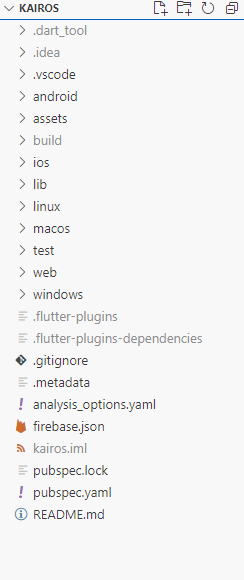
\includegraphics[width=0.5\linewidth]{img/directorios.png}
    \caption{Diseño de aplicar a una subasta y predicción de precio}
    \label{fig:directorios}
\end{figure}

	En la carpeta \emph{assets} se encuentran arhivos de diversos tipos que son necesarios para la realización de la aplicación. En mi caso, la carpeta contiene los siguientes archivos:
	\begin{enumerate}
		\item \textbf{databasewatches.csv :} archivo de extensión csv utilizado para el entrenamiento del modelo de predicción de precios y para cargar los desplegables de campos como \emph{brand}, \emph{model} y \emph{condition} entre otros. Más adelante veremos como se ha conseguido tal tarea.
		\item \textbf{kairoswallpaper.png :} imagen utilizada para establecer el fondo decorativo de la aplicación.
	\end{enumerate}
	
	En la carpeta \emph{lib} encontramos los scripts que han dado vida a la aplicación. Dentro de ella se han creado subdirectorios para seguir un orden y estructura claro. En este caso, los directorios han sido:
	\begin{enumerate}
		\item \textbf{models:} recoge los modelos de la aplicación.
		\item \textbf{views:} recoge los scripts con las vistas y controladores de la aplicación.
		\item \textbf{settings:} recoge scripts con funciones necesarias para traer datos de archivos presentes en la carpeta \emph{assets}.
	\end{enumerate}
	
	Por último, uno de los archivos más importantes es \emph{pubspec.yaml}, donde se definen todas las dependencias con sus versiones necesarias para compilar el programa.

\section{Manual del programador}

	Una vez explicado todo lo que uno debe saber antes de adrentarse en el proyecto, se procede a explicar cómo se ha programado la aplicación.
	
	En la carpeta \emph{models} se encuentran los tres scripts con extensión ``.dart'' que hacen el papel de modelos. Ya se pudo ver en la Figura \ref{fig:db5} y la Figura \ref{fig:db6} que era necesario entablar la comunicación con la base de datos y cómo debía hacerse.
	
	Con esto visto, solo queda explicar las clases ``AuctionRepository'', ``UserRepository'' y ``WatchRepository''. Todas estas clases manejan las operaciones de creación, lectura, actualización y eliminación de objetos según se necesitó para afrontar los requisitos establecidos. Sin embargo, una cosa fundamental que comparten las tres es la instancia de Firebase Firestore dentro de la clase para poder llevar todas estas a cabo, tal y como se representa en la Figura \ref{fig:instanciaFirebase}.

\imagen{instanciaFirebase}{Definición de atributo Firestore}

	Ya que todas las funciones están comentadas y explicar todo haría de este informe una novela, me quiero quedar con cómo se han realizado funciones de consulta de datos a la base de datos. En el caso del modelo ``user.dart'', se necesitó una función que devolviese el dinero de un usuario pasando como parámetro el correo electrónico de este, tal y como se representa en la Figura \ref{fig:consultaMonedero}.
	
\imagen{consultaMonedero}{Forma de consulta de datos a base de datos}

	La forma de consultar datos a base de datos nos obliga, en este caso, a definir una función asíncrona que devolverá eventualmente un entero. En cuanto a la parte de la consulta, se debe especificar la colección a la que se quiere acceder (recordemos que lo que siempre hemos conocido como tablas, aquí son colecciones), la condición que debe cumplir, y limitamos a uno el resultado porque solo debemos recibir un único valor (en este caso la cantidad del dinero asociado a ese correo electrónico). El ``.get()'' será el encargado de devolvernos un ``QuerySnapshot'' con los resultados de la consulta. 
	
	La siguiente comprobación simplemente nos asegura que, si ``QuerySnapshot'' no llegó vacío, devuelva el valor \emph{wallet} del primer documento. Si algo hubiera salido mal, se lanzaría una excepción especificando que el usuario no fue encontrado.
	
	Con las cosas claras de la parte de los modelos, pasamos a la parte de \emph{settings}. Como se ha explicado antes, esta carpeta se destinó a albergar funciones que pudieran ser comunes a varios \emph{scripts} y/o comunicaciones con otros archivos. En este caso, se destinó a albergar el \emph{script} donde se encuentra la función que permite cargar y procesar los datos del archivo con extensión ``.csv'' alojado en la carpeta \emph{assets}.
	
	Tal y como se representa en la Figura \ref{fig:cargaCSV}, la función va a cargar el archivo utilizando una función propia de Flutter y va devolver una lista de mapas con los datos procesados. Es importante tener en cuenta que la primera fila del archivo son los encabezados, por lo que se indica con ``csvTable.skip(1)''. 
	
\imagen{cargaCSV}{Función para extraer datos de dataset}

	En cuanto a las vistas, las funciones quedan explicadas en el código con distintos comentarios donde sean necesarios. Sin embargo, existen ciertas funciones que conviene dejar explciadas en este informe por si surgiese cualquier duda.
	
	Como podemos apreciar en la Figura \ref{fig:responsive}, todos los textos, botones e imágenes de la aplicación van a compartir semejanzas con ella. Es cierto que podría haberse utilizado funciones \emph{responsive} propias de la herramienta, pero durante la realización vimos que afeaba la interfaz ya que los botones tendían a ocupar el largo de la pantalla y, en monitor, no quedaba bonito. Por esta razón, se ideó ajustar el tamaño de los distintos objetos antendiendo al largo de la pantalla.
	
\imagen{responsive}{Forma de hacer la aplicación responsive}

	Otro aspecto importante es la actualización de \emph{widgets} cada vez que viajabamos de una vista a otra y/o realizabamos acciones que necesitaran de un \emph{reload} de la ventana para visualizar los nuevos datos. Un caso lo tenemos en la vista ``home.dart'', donde queremos que el \emph{widget} que presenta el dinero del usuario, se actualice cada vez que viajamos a la venta home. Esto es lo que se representa en la Figura \ref{fig:estadoWallet}. 

\imagen{estadoWallet}{Forma de actualizar un widget}

	Muchas de las cosas predefinidas por Flutter no son intuitivas para el usuario, por lo que se pensó definir una función que controlase la forma de visualizar los mensajes informativos que se den a lo largo de la apliación. Para ello se utiliza la función presentada en la Figura \ref{fig:formaDialogos}, la cual consta de dos partes donde definimos el título del error y una descripción detallada de ello.
	
\imagen{formaDialogos}{Funcion para visualización de diálogos}

	Como hemos indicado en otros apartados, la aplicación cuenta con una llamada a una API, consulta que es necesario definir en el \emph{script} ``addwatch.dart''. Para ello, es importante previamente importar el paquete ``http'', el cual va a permitir que podamos lanzar la consulta, indicando la dirección de la API en la web (alojada en Render). Si el estado de la consulta es 200, todo habrá ido bien. En cambio, si no lo fuese, debemos tratar las excepciones tal y como se plantea en el código. Código en la Figura \ref{fig:llamadaAPI}.

\imagen{llamadaAPI}{Forma de hacer consulta a la API}

	En cuanto a las contraseñas, me pareció una buena idea incluir una función muy presente en muchas webs y aplciaciones: ocultar y mostrar la \emph{password}. Para ello, simplemente definí dos variables booleanas que marcaran si la contraseña se debía mostrar o no en función del pulso sobre el botón definido. Tal código se ve representado en la Figura \ref{fig:ocultarPassword} y la Figura \ref{fig:ocultarPassword2} respectivamente.

\imagen{ocultarPassword}{Variables booleanas para contraseña}
\imagen{ocultarPassword2}{Lógica de ocultar y mostrar contraseña}

	Otro concepto que puede no ser entendido es lo definido como ``regex''. Simplemente se conocen como expresiones regulares y su objetivo es marcar patrones para la manipulación de texto. Mediante su uso, se ha conseguido marcar las validaciones de campos como contraseña, número de cuenta o nombre del usuario, entre otros. Su programación de puede ver en la Figura \ref{fig:validaciones}.
	 
\imagen{validaciones}{Expresiones regulares}

	Por último, no me quería dejar una función importante a la hora de establecer los primeros pasos con Firestore Database. En el script ``main.dart'', en la mayoría de casos, solo se recogen las rutas definidas en la aplicación. Sin embargo, al trabajar con esta base de datos, es necesario definir la función representada en la Figura \ref{fig:inicializacionBaseDeDatos} para que todo funcione correctamente.
	
\imagen{inicializacionBaseDeDatos}{Función que inicializa Firebase}


\section{Compilación, instalación y ejecución del proyecto}

	Para poder ejecutar el proyecto en nuestro equipo, es importante cumplir una serie de requisitos previos e instalar algún que otro programa. Para hacerlo de la manera más estructurada posible, se detallan a continuación los que seguí según \cite{instalacion:flutter}:
	
	\begin{enumerate}
		\item Entramos en sitio web oficial de Flutter \cite{flutter}.
		\item Pulsamos sobre el botón ``Get started''.
		\item Pulsamos sobre el icono de nuestro sistema operativo (en mi caso Windows)
		\item Pulsamos sobre el botón ``Mobile''
		\item Instalamos Visual Studio Code como 
	\end{enumerate}
	
	(Falta completarlo)

%	Antes de explicar como poner el proyecto en nuestro ordenador, me gustaría marcar cuáles han sido los pasos seguidos para crear el proyecto. Esto puede ser de ayuda a futuros estudiantes por su alguno de los pasos a seguir desembocan en errores no comprensibles:
%	\begin{enumerate}
%		\item Desde la consola, nos situamos en la carpeta donde queramos crear el proyecto.
%		\item Escribimos flutter create nombredelproyecto
%		\item Nos situamos en el proyecto.
%		\item Escribimos cmd . para abrir VSC
%	\end{enumerate}
%	
%	Estos serían los pasos principales para la creación del proyecto. Una vez realizados, para conectar Flutter a Firebase, es decir, nuestra base de datos realizamos:
%	\begin{enumerate}
%		\item Vamos a Firebase en nuestro navegador
%		\item Iniciamos sesión
%		\item Pulsamos en el apartado Ir a la consola
%		\item Creamos el proyecto con el nombre que se desee
%		\item Habilitamos análisis y seleccionamos España
%		\item Dentro del apartado compilación creamos firestore database
%		\item Pulsamos sobre crear base de datos
%		\item Marcamos como ubicación eur3(Europe)
%		\item Marcamos comenzar en modo de prueba. Recomendable cambiar el campo fecha manualmente para no perder la base de datos.
%	\end{enumerate}
%	
%	De esta forma, ya habríamos creado la base de datos en la nube. Sin embargo, es necesario comunicar esta con nuestra aplicación Flutter. Para ello:
%	\begin{enumerate}
%		\item En consola, nos situamos en la carpeta del proyecto y escribimos flutter pub add $firebase_core$
%		\item Descargamos aplicación node.
%		\item Ejecutamos como administrador el comando npm install -g $firebase-tools$
%		\item Escribimos firebase login e iniciamos sesión
%		\item Escribimos dart pub global activate $flutterfire-cli$
%		\item Escribimos flutterfire configure
%		\item Con las flechas nos situamos en el proyecto, dejamos marcados todos los campos y marcamos yes
%	\end{enumerate}	

\section{Pruebas del sistema}

(Falta completarlo)
\apendice{Documentación de usuario}

\section{Introducción}

\section{Requisitos de usuarios}

\section{Instalación}

\section{Manual del usuario}



\apendice{Anexo de sostenibilización curricular}

%\section{Introducción}
%Este anexo incluirá una reflexión personal del alumnado sobre los aspectos de la sostenibilidad que se abordan en el trabajo.
%Se pueden incluir tantas subsecciones como sean necesarias con la intención de explicar las competencias de sostenibilidad adquiridas durante el alumnado y aplicadas al Trabajo de Fin de Grado.
%
%Más información en el documento de la CRUE \url{https://www.crue.org/wp-content/uploads/2020/02/Directrices_Sosteniblidad_Crue2012.pdf}.
%
%Este anexo tendrá una extensión comprendida entre 600 y 800 palabras.


	Mi paso por la Universidad de Burgos no solo me ha ayudado a encontrarle el gusto a un mundo tan grande como la informática, si no que ha sido una transcurso del tiempo donde he podido madurar como persona. Recuerdo el primer curso de la carrera como si fuera ayer. Entré pensando ser conocedor de mucha parte de la informática por ser bueno con los dispositivos electrónicos, pero en tan solo dos semanas me di cuenta de que no conocía ni una décima parte de lo que la informática abarcaba.
	
	Para mí, terminar este trabajo ha sido uno de los logros personales más emocionantes que he experimentado. No solo por saber que es el final, si no por todo lo que ha conllevado. El grado me ha enseñado a mejorar mi trabajo en equipo, cosa que me hizo mejorar en mi vida deportiva. El grado me ha enseñado a aportar soluciones a cualquier problema que me tocara afrontar. Y todo esto se ve reflejado en este trabajo.
	
	Si algo define este proyecto es la constancia a no rendirse en ningún momento. A saber que soy yo quien debía decidir cuando acabar y no los problemas personales externos. A valerme por mi mismo y conseguir desplegar una idea propia con la ayuda de mis tutores, a quien doy las gracias y dedico esta línea para decirles una vez más lo fácil y satisfactorio que ha sido trabajar con ellos.
	
	Centrándome más en lo aprendido durante el grado y aplicado a este trabajo, creo que no sería totalmente objetivo marcando cuáles han sido las asignaturas que más han influido en este proyecto. Creo firmemente que de todas he sacado tanto conocimientos teóricos como enseñanzas para mi futura vida laboral y personal.
	
	En lo que respecta a la parte del \emph{front-end}, debo admitir que la programación \emph{web} ha sido muy escasa a lo largo de estos años. No ha habido ninguna asignatura que se centrase únicamente en ello. Con esto no quiero decir que se deba más importancia a ello, pero si que me parezca extraño que no haya una serie de créditos dedicados a realizar y desplegar una aplicación web, aunque sea mínima. Sin embargo, aquí debo referenciar a la empresa que me dio la oportunidad de realizar mis prácticas curriculares con ellos, pues me enseñaron las bases de todo lo que una aplicación web de tener, sea cual sea.
	
	Aun así, el \emph{front-end} no solo es programar. También se deben realizar unas tareas previas que son de vital importancia a la hora de asentar qué es lo que quiere ver el usuario y cómo podemos hacer para que el usuario se sienta cómodo. Un ejemplo es ``Análisis y Diseño de Sistemas''. Sin embargo, si hablamos más de cómo debemos gestionar un proyecto o definir cuáles son los requisitos que el cliente quiere para su aplicación, asignaturas como ``Ingeniería del Software'', ``Gestión de Proyectos'' o ``Validación y Pruebas'' son ejemplos claros. Me gustaría destacar estas dos últimas por la gran aportación que han tenido tanto en mi Trabajo de Fin de Grado como en mi corta vida laboral.
	
	En cuanto a la parte más técnica, asignaturas como ``Programación'', ``Metodología de la programación'', ``Estructura de datos'', ``Sistemas inteligentes'' o ``Procesadores del lenguaje'' me han aportado muchos conocimientos. Aunque el lenguaje de programación utilizado en este proyecto es totalmente distinto a lo visto en estas asignaturas, el profesorado ha conseguido que asiente las bases de la programación. Además, como confesión personal, a veces de tanto programar he adquirido la manía de imaginarme lo que veo llevado a la programación y el flujo de datos. Tengo que añadir que, personalmente, junto con las asignaturas ``Sistemas operativos'' y ``Informática Básica'', han sido un verdadero reto y me han servido en mi vida personal para no rendirme nunca y saber que con trabajo se consigue cualquier cosa que uno se proponga, y una de ellas es este proyecto.
	
	Por otro lado, si nos centramos en la parte \emph{back-end} del proyecto, las asignaturas ``Bases de datos'' y ``Aplicaciones de Bases de Datos'' han sido las claras protagonistas en esta parte del trabajo. A título personal, encontré en estas asignaturas un mundo que desconocía y que hoy es una de mis ramas preferidas dentro de la informática. Aunque son solo dos asignaturas frente a las casi cuarenta disponibles, la cantidad de conocimientos sobre bases de datos adquirida por mi persona es notable. En cuanto al trabajo, como ya se ha indicado en anteriores apartados, la naturaleza de la base de datos no correspondía con las SQL utilizadas mayoritariamente en estas. Sin embargo, esto no ha sido un impedimento y se ha resuelto todo sin mayor problema.
	
	Por último, me gustaría destacar una experiencia que marcó un antes y un después en mi etapa universitaria: el programa ERASMUS. Para mí, fue una etapa de madurez estudiantil impresionante, no solo por el aprendizaje y mejora de distintos idiomas, si no por ver la importancia de estudiar y finalizar una carrera como Ingeniería Informática.


\bibliographystyle{plain}
\bibliography{bibliografiaAnexos}

\end{document}
